%-------------------------------------------------------------
\section{$^{85}$Kr in liquid xenon}
\label{secKr85}

Commercially available xenon gas, where purification is performed by distillation and adsorption-based chromatography, has a concentration of natural krypton at the ppm level.
Natural krypton contains about 10$^{-11}$~g/g of radioactive $^{85}$Kr. 
The background from the beta decay of $^{85}$Kr, with T$_{1/2}$ = 10.76~years and endpoint energy 687~keV, is a potential limitation in the sensitivity of rare-event searches using xenon targets.

The gas used in the XENON100 experiment has been processed at a commercial distillation plant to reduce the concentration of krypton to $<$10~ppb.
The high-temperature getter used in the experiment to purify xenon from water and electronegative contaminants does not remove the noble gas krypton. Therefore, an additional gas purification has been performed with cryogenic distillation. The reduction of krypton concentration down to a few ppt has been reported in Ref.~\cite{distillation}, with a distillation column similar to the one procured by XENON100.



%-------------------------------------------------------------
\subsection{Measurement of krypton concentration in liquid xenon with delayed coincidence analysis}

The level of krypton in the LXe has been measured with a delayed coincidence analysis using a decay channel where $^{85}$Kr undergoes a $\beta$-decay with E$_{max}$~=~173.4~keV to $^{85m}$Rb, which in turn decays to the ground state with T$_{1/2}$~=~1.015~$\mu$s emitting a $\gamma$-ray with an energy of 514~keV. The branching ratio of this decay channel is 0.434\%, which makes this method insensitive to low concentrations of krypton.

The concentration of $^{nat}$Kr in the LXe determined with this technique is 143$_{-90}^{+130}$~ppt [mol/mol], assuming a $^{85}$Kr abundance of 10$^{-11}$.

The light yield of 2.0 and 1.6 phe/keV$_{ee}$ has been assumed for the 1st and 2nd S1 peaks.
The detector resolution using S1 signal only can be described with the function $\frac{1}{E [MeV]}$~+~11.2\%. Using this formula, resolution at 173 (the endpoint energy of the electron) and 514~keV (mean energy of the gamma) is 13.6\% and 12.6\%, respectively. The resulting energy range to select events from $^{85}$Kr decay is from 40 to 220 phe.


%-------------------------------------------------------------
\subsection{Background from $^{85}$Kr decay}

Levels of radioactive trace contaminations in xenon might vary at different stages of the experiment, as they strongly depend on purification processes. The background rate from intrinsic radioactivity in LXe has thus been predicted for different  concentrations of $^{nat}$Kr in LXe, and is shown in Figure~\ref{figLXeKr}.

Another intrinsic source of background is the decay of $^{222}$Rn daughters in the LXe. Radon is present in the LXe due to emanation from detector materials and the getter, and diffusion of the gas  through the seals. 

In the Monte Carlo simulation, $^{222}$Rn decays are generated uniformly in the LXe, and only the part of the chain before $^{210}$Pb is considered, since the relatively long half-life time of 22.3 years for $^{210}$Pb results in radioactive disequilibrium in the decay chain.
The predicted background rate in the energy region below 100~keV is shown in Figure~\ref{figLXeRn} as a function of the $^{222}$Rn concentration in the LXe.

\begin{figure}[!h]
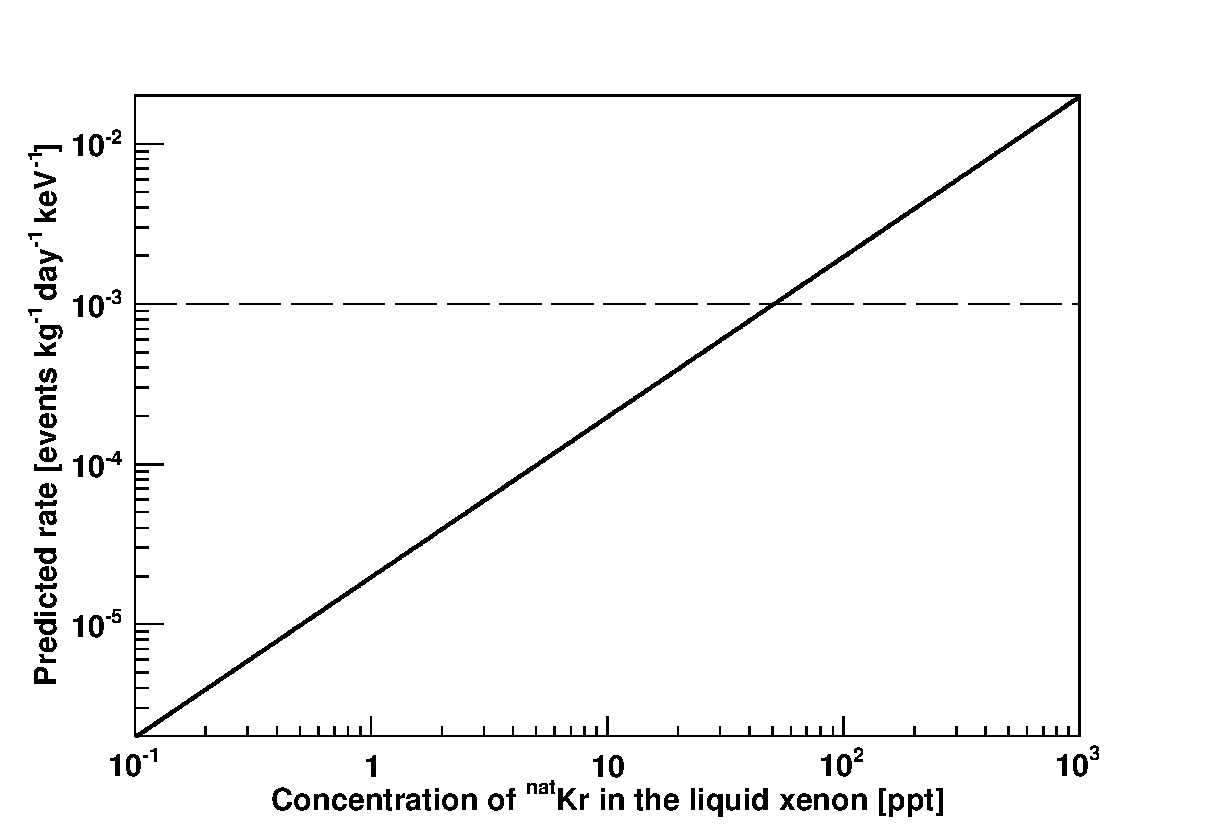
\includegraphics[width=0.7\linewidth]{plots/Kr85/Kr85_Rate-vs-Conc.eps}
\caption[Rate of single electronic recoils from $^{85}$Kr decay]{Rate of single electronic recoils from $^{85}$Kr decay in the energy region below 100~keV as a function of the concentration of natural Kr in the LXe. Fiducial and veto cuts are inefficient for this intrinsic background source. As a reference value, the horizontal dashed line corresponds to a background rate of 10$^{-3}$~events$\cdot$kg$^{-1}\cdot$day$^{-1}\cdot$keV$^{-1}$. }
\label{figLXeKr}
\end{figure}



